% Primary source: https://github.com/cra-ros-pkg/robot_localization/blob/rolling-devel/doc/state_estimation_nodes.rst
% Primary source: https://index.ros.org/p/robot_localization/
\documentclass[tikz,border=5pt]{standalone}
\usepackage[T1]{fontenc}
\usepackage{lmodern,amsmath,amssymb}
\usetikzlibrary{arrows.meta,calc,positioning,fit,backgrounds,shapes.geometric,matrix,decorations.pathreplacing,patterns}
\definecolor{ink}{gray}{0.08}
\definecolor{wash}{gray}{0.965}
\definecolor{soft}{gray}{0.45}
\tikzset{box/.style={draw=ink,line width=.65pt,fill=white,align=center,inner sep=4pt,outer sep=0pt,font=\small},flow/.style={draw=ink,line width=.65pt,-{Latex[length=1.8mm,width=1.3mm]},rounded corners=2pt},annotation/.style={font=\scriptsize,text=soft,align=center},groupbox/.style={draw=soft,dashed,line width=.45pt,fill=wash}}
\begin{document}
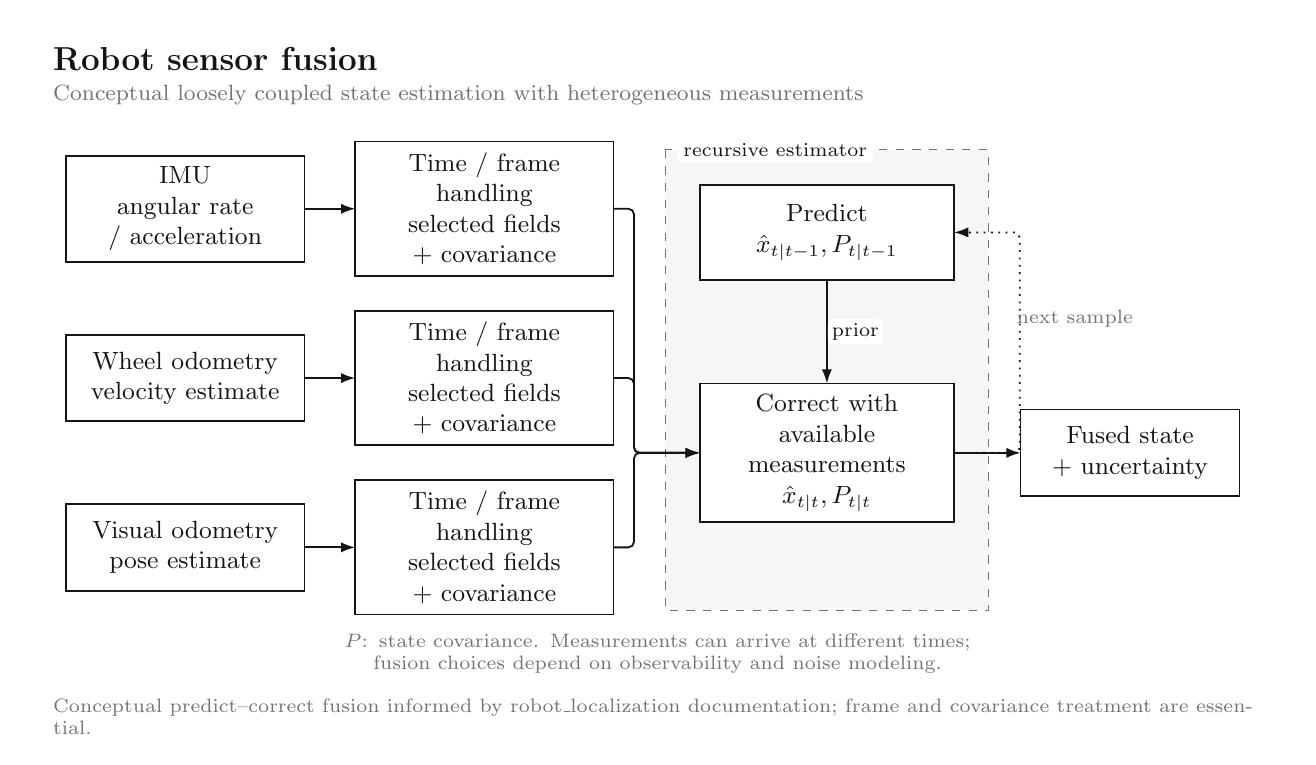
\begin{tikzpicture}[x=1cm,y=-1cm,font=\rmfamily,text=ink]

\path[use as bounding box] (0,0) rectangle (16,9);
\node[anchor=west,font=\large\bfseries] at (.2,.4) {Robot sensor fusion};
\node[anchor=west,font=\footnotesize,text=soft] at (.2,.85) {Conceptual loosely coupled state estimation with heterogeneous measurements};
\begin{pgfonlayer}{background}
\draw[groupbox] (8.1,1.55) rectangle (12.2,7.3999999999999995);
\node[anchor=west,font=\scriptsize,fill=white,inner sep=2pt] at (8.25,1.55) {recursive estimator};
\end{pgfonlayer}
\node[box,minimum width=3.0cm,minimum height=1.1cm,text width=2.75cm] (imu) at (2.0,2.3) {IMU\\angular rate / acceleration};
\node[box,minimum width=3.25cm,minimum height=1.1cm,text width=3.0cm] (imuprep) at (5.8,2.3) {Time / frame handling\\selected fields + covariance};
\node[box,minimum width=3.0cm,minimum height=1.1cm,text width=2.75cm] (wheel) at (2.0,4.45) {Wheel odometry\\velocity estimate};
\node[box,minimum width=3.25cm,minimum height=1.1cm,text width=3.0cm] (wheelprep) at (5.8,4.45) {Time / frame handling\\selected fields + covariance};
\node[box,minimum width=3.0cm,minimum height=1.1cm,text width=2.75cm] (vision) at (2.0,6.6) {Visual odometry\\pose estimate};
\node[box,minimum width=3.25cm,minimum height=1.1cm,text width=3.0cm] (visionprep) at (5.8,6.6) {Time / frame handling\\selected fields + covariance};
\node[box,minimum width=3.2cm,minimum height=1.2cm,text width=2.95cm] (predict) at (10.15,2.6) {Predict\\$\hat{x}_{t|t-1},P_{t|t-1}$};
\node[box,minimum width=3.2cm,minimum height=1.45cm,text width=2.95cm] (correct) at (10.15,5.4) {Correct with available\\measurements\\$\hat{x}_{t|t},P_{t|t}$};
\node[box,minimum width=2.75cm,minimum height=1.1cm,text width=2.5cm] (output) at (14.0,5.4) {Fused state\\+ uncertainty};
\begin{pgfonlayer}{background}
\draw[flow] (imu.east) -- (imuprep.west);
\draw[flow] (wheel.east) -- (wheelprep.west);
\draw[flow] (vision.east) -- (visionprep.west);
\draw[flow] (predict.south) -- (correct.north) node[midway,right,fill=white,inner sep=1.5pt,font=\scriptsize] {prior};
\draw[flow] (imuprep.east) -- (7.7,2.3) -- (7.7,5.4) -- (correct.west);
\draw[flow] (wheelprep.east) -- (7.7,4.45) -- (7.7,5.4) -- (correct.west);
\draw[flow] (visionprep.east) -- (7.7,6.6) -- (7.7,5.4) -- (correct.west);
\draw[flow] (correct.east) -- (output.west);
\draw[flow,dotted] (correct.east) -- (12.6,5.4) -- (12.6,2.6) -- (predict.east);
\end{pgfonlayer}
\node[annotation,text width=2.0cm] at (13.3,3.7) {next sample};
\node[annotation,text width=14.3cm] at (8.0,7.95) {$P$: state covariance. Measurements can arrive at different times; fusion choices depend on observability and noise modeling.};
\node[anchor=west,align=left,font=\scriptsize,text=soft,text width=15.6cm] at (.2,8.75) {Conceptual predict--correct fusion informed by robot\_localization documentation; frame and covariance treatment are essential.};
\end{tikzpicture}
\end{document}
